\chapter{Literature Review}
\label{ch:background}

\section{A History of DeepFakes}

% \begin{itemize}
%     \item More detailed explanation of deepfakes
%     \item How are they generated
%     \begin{itemize}
%         \item GANs
%         \item assorted other AI shenanigans
%     \end{itemize}
% \end{itemize}

\subsection{Photo Manipulation}

Humans have been manipulating photographs since the 1860s. The first known example of photographic manipulation was when a photo of United States President Abraham Lincoln was composited onto fellow politician John Calhoun's body\cite{singh2018art}, shown in Figure \ref{fig:lincoln}. Photo tampering was then used throughout history as a way to shape the opinions and beliefs of individuals by altering supposed ``evidence". As photography was still an entirely analogue process, editing a photo was significantly harder than it is today; nevertheless, it was still done when deemed necessary. Another famous example is the removal of Nikolai Yezhov in 1940 from a 1937 photo with Joseph Stalin after the ``Great Purge" in the Union of Soviet Socialist Republics (Figure \ref{fig:stalin-yezhov}).

\begin{figure}[H]
    \centering
    \begin{subfigure}{0.45\textwidth}
            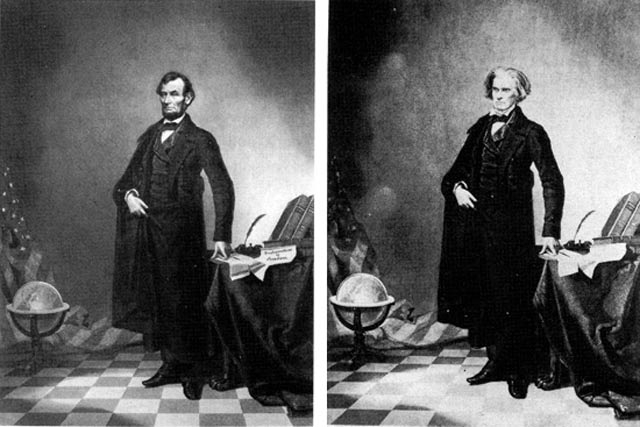
\includegraphics[width=\textwidth]{dissertation//figures/lincoln1960.jpg}
            \caption{A spliced portrait of Abraham Lincoln (left) with the original (right)\cite{singh2018art}}
            \label{fig:lincoln}
    \end{subfigure}
    \begin{subfigure}{0.45\textwidth}
        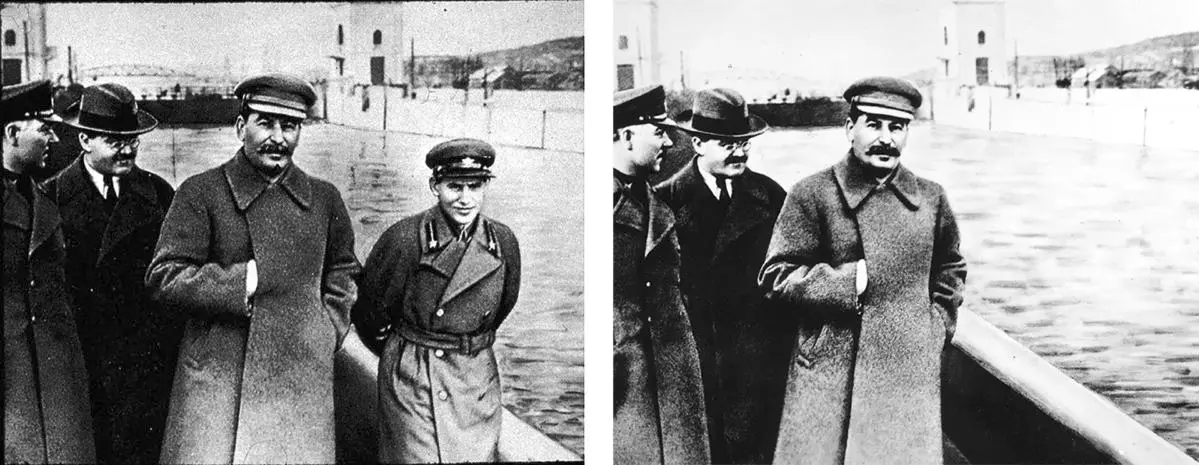
\includegraphics[width=\textwidth]{dissertation//figures/stalin.png}
        \caption{A photo of Stalin and Yezhov (left) which was subsequently edited to remove Yezhov (right)}
        \label{fig:stalin-yezhov}
    \end{subfigure}
    \caption{Examples of historical images that were edited}
    \label{fig:edited-images}
\end{figure}

With the advent of digital photography and computers, photo manipulation became available to the general public. Suddenly, images were not physical items but data stored on a computer, which could be easily manipulated. Changes could be viewed instantly, reversed, and shared easily. Programs to edit images were released, such as Adobe Photoshop\footnote{\url{https://www.adobe.com/uk/products/photoshop.html}} and GIMP\footnote{\url{https://www.gimp.org/}}. Although these tools made photo editing cheap and accessible, they still required time, effort, and skill from humans in order to produce a convincing forgery. An original image is also required for manipulation.

Computer Generated Imagery (CGI) is a technique primarily used in movies to artificially augment a frame, often with completely novel additions. CGI was first used in the 1958 film ``Vertigo" and became widespread in the 1990s\cite{ozturk2023vicious}. Presently, CGI is used in almost every major film to generate realistic images. In ``Rogue One: A Star Wars Story" the actor Peter Cushing digitally recreated after his death in 1994 to play Grand Moff Tarkin posthumously(Figure \ref{fig:tarkin}). While CGI requires large amounts of computational resources, consumer-grade image generation which runs on much worse hardware has equally progressed. Most modern social media apps contain a variety of beauty filters\cite{corcoran2014digital}. For example, a blur can be applied to reduce skin blemishes as shown by Figure \ref{fig:beauty-filter}. These are often less computationally expensive and can run on smartphones and other edge devices, offering the ability to manipulate media to the masses, not just the technically able and skilled.

\begin{figure}[H]
    \centering
    \begin{subfigure}{0.45\textwidth}
        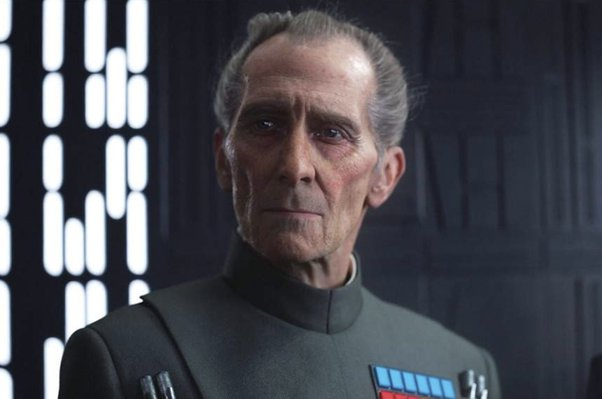
\includegraphics[width=\linewidth]{dissertation//figures/grandmoff-tarkin.jpg}
        \caption{A digital recreation of Peter Cushing for the film ``Rogue One: A Star Wars Story"\cite{rogueone}}
        \label{fig:tarkin}
    \end{subfigure}
    \begin{subfigure}{0.45\textwidth}
        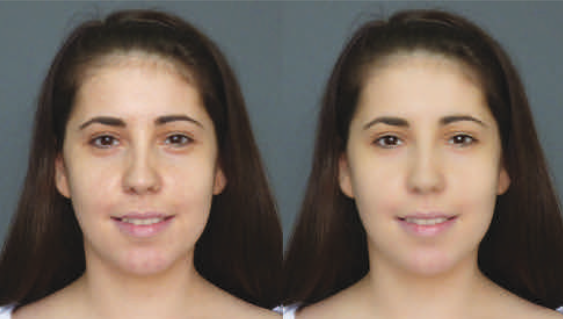
\includegraphics[width=\linewidth]{dissertation//figures/blurring.png}
        \caption{An original image (left) blurred to remove skin blemishes (right)\cite{corcoran2014digital}}
        \label{fig:beauty-filter}
    \end{subfigure}
    \caption{Examples of digital image manipulation}
    \label{fig:digital-manipulation}
\end{figure}

\subsection{Artificial Intelligence for Manipulating Media}

\subsubsection{Neural Networks}

DeepFakes are a subset of neural networks. Neural networks are a subsection of AI which imitate the structure of a brain to perform computations\cite{islam2019overview}. Traditional computation manipulates binary data, whereas neural networks manipulate the connections between fixed binary elements. Work on simulating the brain using mathematical functions began in 1920\cite{brush1967history}, 37 years before the academic formalisation of AI in 1957 at the Dartmouth Workshop\cite{crevier1993ai}. The field would remain relatively stagnant until the proposal of the Multi-Layer Perceptron (MLP) in 1958\cite{rosenblatt1958perceptron} and how it could ``learn" in 1967\cite{ivakhnenko1967cybernetics}.

Neural networks contain a collection of neurons organised into layers, each layer receives inputs from the neurons earlier in the network (Figure \ref{fig:full-neural-network}). Each of the $n$ inputs to a nueron has an associated weight ($w_i$) and value ($x_i$). Once the combined weights and an additional bias weight ($b$) exceed a determined threshold (usually 0), then the neuron fires with an output ($y$) determined by an activation function ($f(x)$). This is shown in Equation \ref{eq:neuron-activation} and Figure \ref{fig:neural-network}. The network shown in Figure \ref{fig:neural-network} has a one-dimensional input, however, MLPs can expand to an infinite number of dimensions.

\begin{equation}
\label{eq:neuron-activation}
    \begin{array}{c@{\hspace{2cm}}c}
        W = b+\displaystyle\sum_{i=1}^{n} w_ix_i  &
        y = \begin{cases}
            f(W) & \text{if } W \geq 0  \\
            0/-1 & \text{otherwise}
        \end{cases}
    \end{array}
\end{equation}

\begin{figure}[H]
    \centering
    \begin{subfigure}{0.45\textwidth}
        \centering
        \begin{tikzpicture}
            % inputs
            \node[draw=none] (x1) at (-1,2) {\(x_1\)};
            \node[draw=none] (x2) at (-1,0) {\(x_2\)};
            \node[draw=none] (x3) at (-1,-2) {\(x_3\)};
            
            % nuron (split circle)
            \node[draw, circle, minimum size=1.8cm, thick] (neuron) at (3,0) {};
            \node at (2.5, 0) {\(\sum\)}; % Left side - Summation
            \node at (3.5, 0) {\(f\)}; % Right side - Activation
            \draw[thick] (neuron.south) -- (neuron.north); % dividing line
            
            % output
            \node[draw=none] (output) at (6,0) {\(y\)};
            \draw[->] (neuron.east) -- (output);
            
            % weights
            \draw[->] (x1) -- node[above] {\(w_1\)} (neuron.west);
            \draw[->] (x2) -- node[above] {\(w_2\)} (neuron.west);
            \draw[->] (x3) -- node[below] {\(w_3\)} (neuron.west);
            
            % bias
            \node[draw=none] (bias) at (3,-2.5) {\(b\)};
            \draw[->] (bias) -- (neuron.south);
        \end{tikzpicture}
        \caption{Structure of a single artificial neuron}
        \label{fig:neuron}
    \end{subfigure}
    \begin{subfigure}{0.45\textwidth}
        \centering
        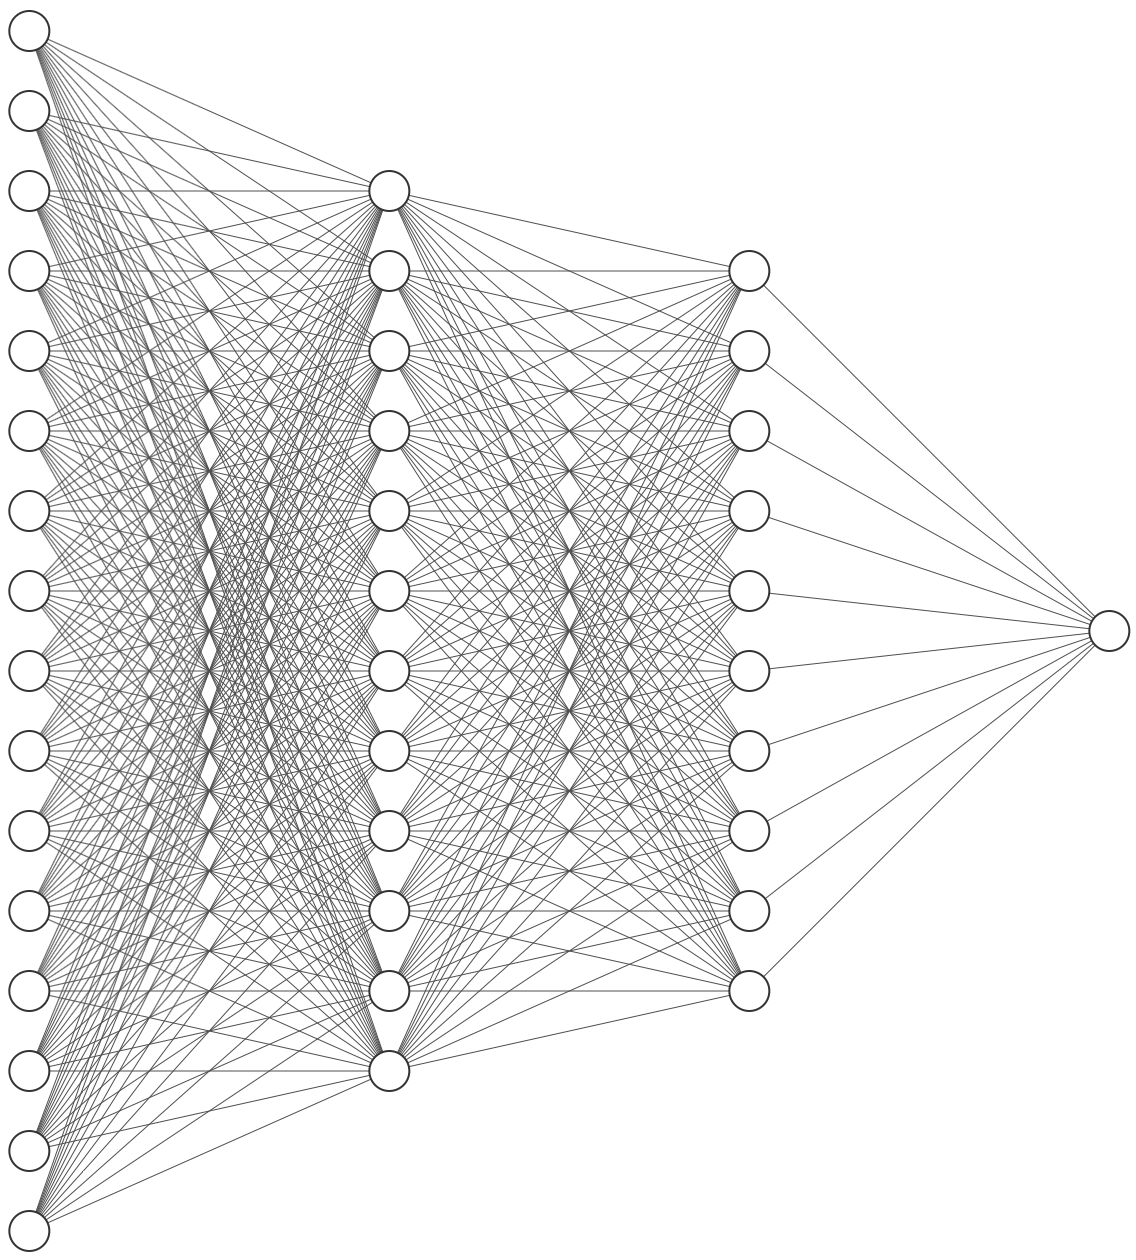
\includegraphics[width=0.75\textwidth]{dissertation//figures/generic-neural-diagram.png}
        \caption{A network of neurons split into layers}
        \label{fig:full-neural-network}
    \end{subfigure}
    \caption{A structure of a neural network and the individual neurons within it}
    \label{fig:neural-network}
\end{figure}

Neural networks are able to learn. When given a set of labelled data, it is possible for a neural network to use specialised algorithms to adjust the weights and biases in the network so that the final output is similar to the labels provided. A detailed explenation of learning is provided in Section \ref{sec:learning}

\subsubsection{Convolutional Neural Networks}
\label{sec:cnns}

Although MLPs are exceptionally versatile, they can suffer from overfitting. Overfitting is where a machine learning model learns the training data but not a general solution, becoming exceptionally accurate in the training data, but underperforming on test data. With every neuron in an MLP layer being connected to all other neurons in the layers ahead and behind it, the network is prone to overfitting\cite{o2015introduction}. A variety of methods can be employed to reduce overfitting, but the most common way is to remove connections from the network by reformatting the layers, this also has the attractive benefit of quicker computations as there are fewer weights to sum resulting in faster training and inference times. Several methods to reduce connections have been proposed, but the most prominent are Convolutional Neural Networks (CNNs).

A CNN is a sequence of three layers: convolution layers, pooling layers, and fully connected layers\cite{ibmconvolutional}. Each set of layers reduces the dimensions of the input, allowing each subsequent layer to take into account a larger portion of the image.

\begin{itemize}
    \item \textbf{Convolutional Layer}\\
    A Convolutional Layer is what a CNN lends its name to. It has two stages. The first stage is a filtering stage, a kernel (sometimes called a filter) is passed over the input. The kernel is placed over a section of the input and the dot product between the values in the kernel and the input is calculated. This then becomes the input to the next layer. The kernel is then shifted over by a fixed stride value to analyse another subset of the input. This process is shown in Figure \ref{fig:filter}. The values (or weights) of each filter remain constant as it moves across the image; there can also be many filters, increasing the dimension of an input. The weights are what are learnt by this layer. Reducing the values to be trained to the size of the filter significantly speeds up the training process. Often some activation layer will be included to process the output matrix. More often than not, this uses the Rectified Linear Unit (ReLU) function, to limit outputs to strictly positive in order to introduce linearity and prevent the vanishing gradient problem (which can hinder learning)\cite{ibmconvolutional}.
    
    \begin{figure}[H]
        \centering
        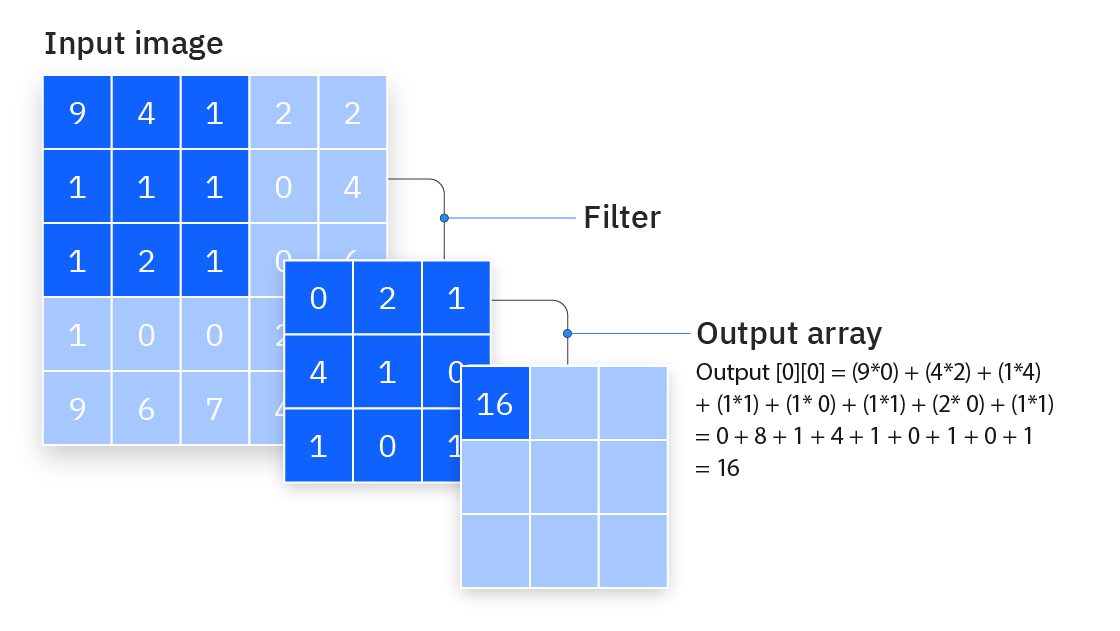
\includegraphics[width=0.5\linewidth]{dissertation//figures/cnn-filter.png}
        \caption{A diagram showing the action of a $3 \times 3$ filter\cite{ibmconvolutional}}
        \label{fig:filter}
    \end{figure}

    \item \textbf{Pooling Layer}\\
    The Pooling Layer is similar to the convolution layer but with no learnable parameters. Instead of a weighted kernel, an aggregation function pools multiple values into a single value\cite{o2015introduction}. Any function could be used, but the most common ones are: max pooling where the maximum value under the kernel is selected; or average pooling where the average of all the values is chosen. Pooling layers further reduce the number of learning parameters: reducing overfitting, model complexity, and computation time\cite{ibmconvolutional}.

    \item \textbf{Dense Layer}\\
    To produce an output that is usable, a final dense layer is needed to convert the output of the previous layers into a desired shape. This is a fully connected MLP network. Often these will be referred to as dense or fully connected layers as every neuron is connected to every other neuron.
\end{itemize}

A sequence of these layers are combined to produce a network. The exact sequence and order is defined by the network's architect and depends on the quality of output they want. More layers mean a higher probable accuracy, but incurs increased computation costs and tendency to overfit. Further techniques exist to enhance CNNs such as skip connections, which results in the output of layers to ``skip" forward layers and act as the input for layers further down the network. An example of a CNN for classifying images is shown in Figure \ref{fig:sample-cnn}:

\begin{figure}[H]
    \centering
    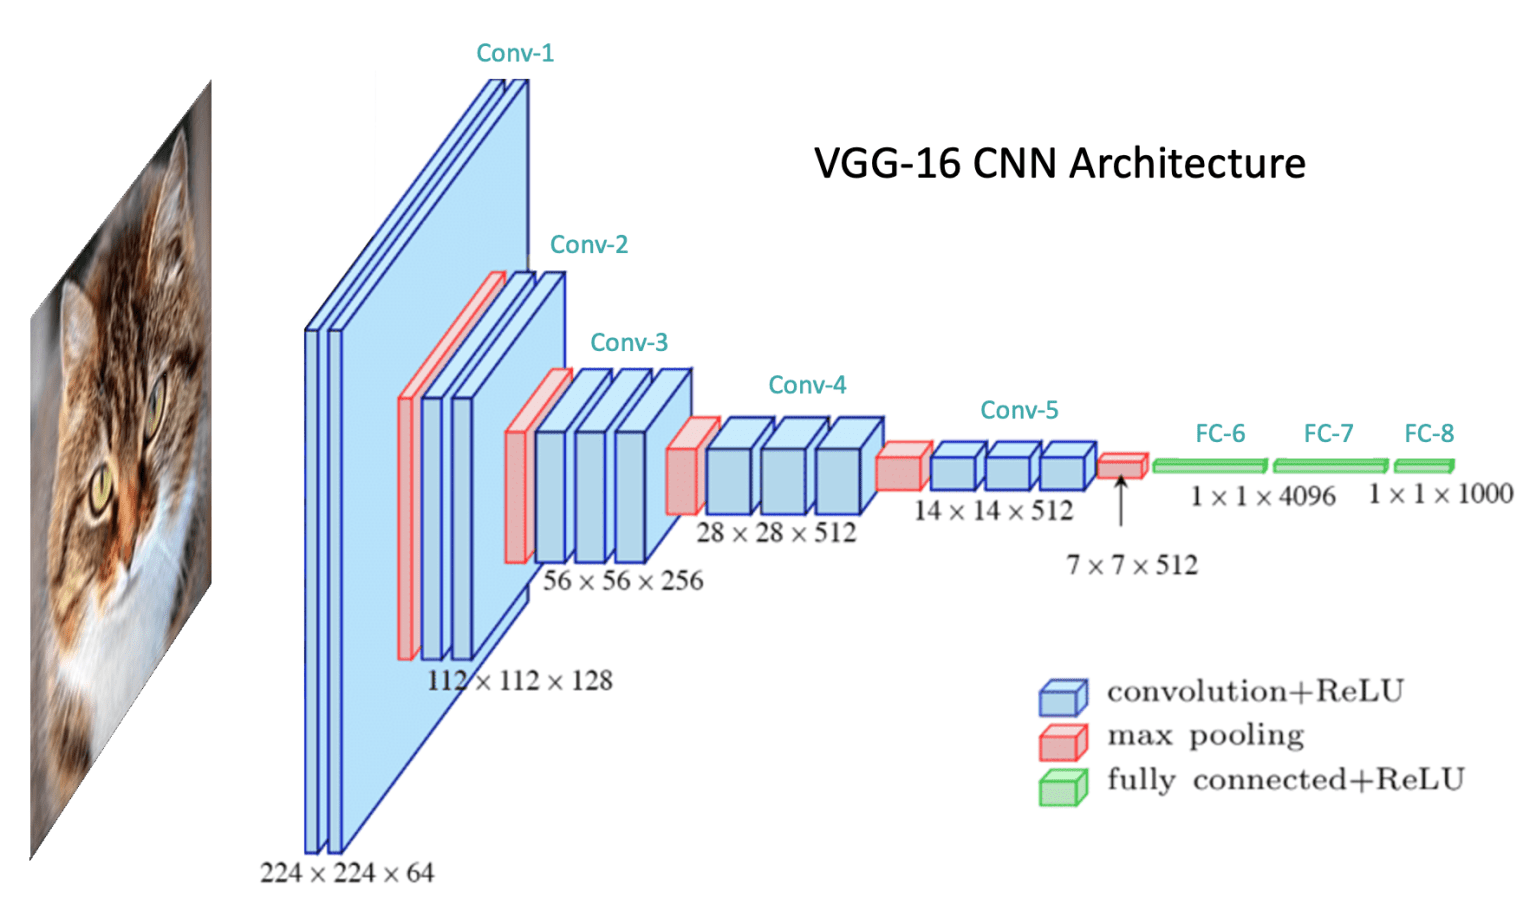
\includegraphics[width=0.5\linewidth]{dissertation//figures/sample-cnn.png}
    \caption{A sample CNN\cite{kromydas2023convolutional}}
    \label{fig:sample-cnn}
\end{figure}

\subsubsection{Learning}
\label{sec:learning}

The process of learning is similar across all kinds of neural networks. Every network will have trainable parameters (the kernel in a convolutional layer or the weights and biases in an MLP) which are initialised randomly. All learnable parameters are then trained in CNNs via backward propagation of error (commonly shortened to backpropagation)\cite{rojas2013neural}.

This method of training requires a train set: a set of inputs and their known correct outputs (sometimes called labels). The backpropagation algorithm proceeds as follows:

\begin{enumerate}
    \item Each input is passed through the network in a forward pass. This produces one or more outputs.
    \item The predicted outputs are compared to the known truth outputs. A user-defined loss function evaluates how ``correct" the network's predictions are, producing a single value. Common loss functions are categorical cross-entropy for classification tasks and Mean Squared Error (MSE) for location problems\cite{begmann-backpropagation}
    \item A backwards pass is then performed to compute the gradients of the loss function with respect to each learnable parameter. Every parameter $x$ in the network is connected to the output through a composite function $f(x)$, incorporating all relevant activation functions and weights. By applying the chain rule and computing the partial derivative ($\frac{\partial L}{\partial x}$ where $L$ is the loss function), it can be ascertained how much each parameter influences the overall error.
\end{enumerate}

For every parameter, how the loss function varies when $x$ is varied can be expressed as a graph (Figure \ref{fig:loss-graph}). By finding the value of $x$ that minimises the loss function for each parameter in the network, the network's accuracy can be improved. Note that the graph will often be more complex, compromising of a variety of hills, valleys, and plateaus.

\begin{figure}[H]
    \centering
    \begin{tikzpicture}
        % graph axis
        \draw[->] (0,0)--(3,0) node[midway,below]{$x$};
        \draw[->] (0,0)--(0,3) node[midway,left]{loss};
        %line
        \draw[domain=0.1:2.9] plot(\x,{(\x-1.5)^2+0.5});
    \end{tikzpicture}
    \caption{A sample plot of the value of the loss function over varying values of a parameter $x$}
    \label{fig:loss-graph}
\end{figure}

A variety of methods exist to find the minimum value for $x$ in the least possible steps. The most widely used is Stochastic Gradient Descent (SGD)\cite{robbins1951stochastic}, first applied to neural networks in 1967\cite{shunichi1967theory}. SGD follows the following formula:

\begin{equation}
    x_n=x_{n-1}-\alpha l(x)
\end{equation}

$x_n$ is the new value of parameter $x$ which had a previous value $x_{n-1}$. The value is altered by $l(x)$, the gradient produced by backpropagation for $x$. $\alpha$ is the learning rate, a hyperparameter. Often a number close to 0, this limits how much the value can vary within the graph. Too low of a learning rate results in slow learning and the potential to get stuck in local minima or plateaus. A high learning rate leads to the possibility of divergence and the minimum never being found.


\begin{figure}[H]
    \centering
    \begin{subfigure}{0.3\textwidth}
        \centering
        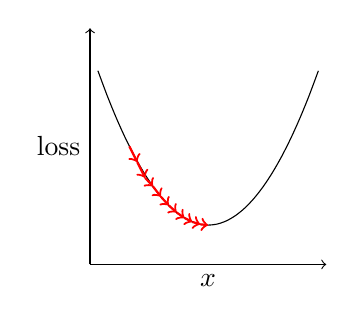
\begin{tikzpicture}
            % graph axis
            \draw[->] (0,0)--(3,0) node[midway,below]{$x$};
            \draw[->] (0,0)--(0,3) node[midway,left]{loss};
            % loss curve
            \draw[domain=0.1:2.9,smooth] plot(\x,{(\x-1.5)^2+0.5});
            % small steps
            \draw[->,red,thick] (0.5,1.5) -- (0.6,1.3);
            \draw[->,red,thick] (0.6,1.3) -- (0.7,1.1);
            \draw[->,red,thick] (0.7,1.1) -- (0.8,0.99);
            \draw[->,red,thick] (0.8,0.99) -- (0.9,0.86);
            \draw[->,red,thick] (0.9,0.86) -- (1.0,0.75);
            \draw[->,red,thick] (1.0,0.75) -- (1.1,0.66);
            \draw[->,red,thick] (1.1,0.66) -- (1.2,0.59);
            \draw[->,red,thick] (1.2,0.59) -- (1.3,0.54);
            \draw[->,red,thick] (1.3,0.54) -- (1.4,0.51);
            \draw[->,red,thick] (1.4,0.51) -- (1.5,0.5);
        \end{tikzpicture}
        \caption{Too low learning rate}
    \end{subfigure}
    \hfill
    \begin{subfigure}{0.3\textwidth}
        \centering
        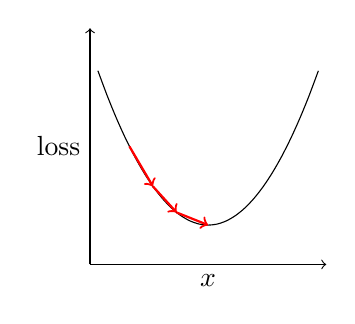
\begin{tikzpicture}
            % graph axis
            \draw[->] (0,0)--(3,0) node[midway,below]{$x$};
            \draw[->] (0,0)--(0,3) node[midway,left]{loss};
            % loss curve
            \draw[domain=0.1:2.9,smooth] plot(\x,{(\x-1.5)^2+0.5});
            % optimal steps
            \draw[->,red,thick] (0.5,1.5) -- (0.8,0.99);
            \draw[->,red,thick] (0.8,0.99) -- (1.1,0.66);
            \draw[->,red,thick] (1.1,0.66) -- (1.5,0.5);
        \end{tikzpicture}
        \caption{Optimal learning rate}
    \end{subfigure}
    \hfill
    \begin{subfigure}{0.3\textwidth}
        \centering
        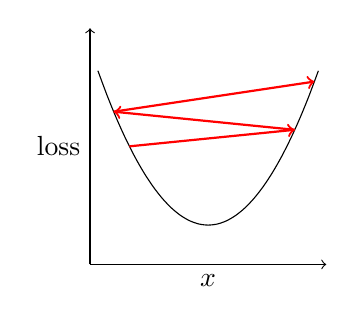
\begin{tikzpicture}
            % graph axis
            \draw[->] (0,0)--(3,0) node[midway,below]{$x$};
            \draw[->] (0,0)--(0,3) node[midway,left]{loss};
            % loss curve
            \draw[domain=0.1:2.9,smooth] plot(\x,{(\x-1.5)^2+0.5});
            % large steps
            \draw[->,red,thick] (0.5,1.5) -- (2.6,1.71);
            \draw[->,red,thick] (2.6,1.71) -- (0.3,1.94);
            \draw[->,red,thick] (0.3,1.94) -- (2.85,2.3225);
        \end{tikzpicture}
        \caption{Too high learning rate}
    \end{subfigure}
    \caption{Effect of different learning rates on loss function optimisation}
    \label{fig:learning-rates}
\end{figure}

Traditionally, finding an optimal learning rate has been a hard problem and thus a variety of methods have been introduced to give a larger safety net when choosing parameters. The most popular of these is the Adaptive Moment Estimator (commonly shortened to Adam)\cite{kingma2014adam}.

Adam combines the advantages of two popular optimisation techniques: adaptive learning rates and momentum. Inspired by AdaGrad \cite{duchi2011adaptive} and RMSProp, Adam maintains a per-parameter learning rate that adapts based on the first and second moments of the gradients. The adaptive learning rate allows the optimiser to apply larger updates for infrequently updated parameters and smaller updates for frequently updated ones. Momentum, on the other hand, helps accelerate the optimisation process by keeping track of the previous gradients, thus smoothing the updates and enabling the optimiser to handle complex loss functions easier.

When training, the above process is done for every learnable parameter for every item in the train set. Often, the train set will be too small to enable meaningful learning. To combat this, the set will be iterated over multiple times. One iteration over the entire dataset is referred to as an epoch\cite{begmann-backpropagation}. Often training will be done for a set number of epochs or until the loss function stabilises. 

\subsubsection{Generative Artificial Intelligence}

Whilst editing an image was relatively easy with modern photo editing tools, adding original content to an image was more difficult, requiring specialist expertise. The difficulty is further increased when trying to edit a video as more images need to be edited and stitched seamlessly together in a consistent manner. Generative AI (GenAI) is a form of neural network that can generate novel content. In images, they can augment images to fit a specific goal or, in more recent works, convert written prompts into completely original images and videos.

The first notable GenAI was Generative Adversarial Networks (GANs)\cite{goodfellow2014generative}. GANs are two neural networks that work in opposition to each other, a generator and a discriminator. The training process is a minimax two-player game: when one model loses by a certain amount, the other model gains an equal amount. In the context of image generation, the generator creates novel images based on a dataset; the discriminator is fed a combination of the dataset and the generator's images, attempting to determine their origin. A diagram of a GAN network is shown in Figure \ref{fig:gan-diagram}. The discriminator is a CNN, whereas the generator is a deconvolutional neural network\cite{zeiler2011adaptive}. Deconvolutional neural networks are CNNs but in reverse, where the deconvolution layers convert a single value into a $n \times n$ square of new values. To produce an image, the generator is fed random noise, which it converts into a novel image. Over time, the generator becomes better and better at generating convincing images from noise that fool the discriminator, eventually resulting in images that appear identical to the images from the dataset. 

\begin{figure}[H]
    \centering
    \begin{tikzpicture}[
        rect/.style={rectangle, draw=black, thick, minimum width=2.5cm, minimum height=1cm},
        bigrect/.style={rectangle, draw=black, thick, minimum width=6cm, minimum height=1cm}
    ]
        \node[rect] (nois) {noise};
        \node[rect] (gene) [above=of nois] {generator};
        \node[rect] (data) [above right=of nois] {dataset};
        \path (gene) -- (data) coordinate[midway] (midpoint);
        \coordinate (abovemid) at ($(midpoint) + (0,2cm)$);
        \node[bigrect] (disc) at (abovemid) {discriminator};

        \draw[->] (nois.north) -- (gene.south);
        \draw[->] (data.west) -- (gene.east);
        \draw[->] (gene.north) -- (disc.south -| gene.north);
        \draw[->] (data.north) -- (disc.south -| data.north);
    \end{tikzpicture}
    \caption{A diagram of the network structure of a GAN}
    \label{fig:gan-diagram}
\end{figure}

Even in the original paper, GANs were being used to generate images of humans\cite{goodfellow2014generative}. In 2017, the technology would expand beyond the realm of academia and into the public eye. A user named \verb|u/deepfakes| and others on the internet forum site Reddit\footnote{\url{https://reddit.com}} were discovered to be sharing pornographic material, altered to contain popular celebrities using GANs\cite{cole2018reddit}. Users were taking ``conventional" pornographic videos and using GANs to swap the faces in the original video to famous individuals without their consent. By only generating the face, these networks required less computational power and thus videos could be generated quickly. Following legal pressure, Reddit deleted the forum two months later\cite{cole2018reddit}, but the damage was done: AI had been shown to generate realistic videos of humans semi-autonomously. The media soon caught on to the story using the subreddit's name to coin the new types of videos as ``DeepFakes", a portmanteau of ``Deep Leaning" and ``fake".

Other methods of generating DeepFakes have been developed since GANs. Diffusion\cite{rombach2022high} is a process of removing noise from images based on transformers\cite{vaswani2017attention}. When given random noise, these models can generate completely novel images. When trained on images with text descriptions, images could be generated from natural language prompts. Multiple different companies began making image generation tools such as OpenAI\cite{ramesh2022hierarchical}, Stable Diffusion\cite{stablediffusion2022}, and Midjourney\cite{midjourney2022}. OpenAI would eventually create Sora\cite{brooks2024video} a model that could generate realistic videos from a text prompt. The most recent architecture for image generators is Visual AutoRegressive modelling (VAR)\cite{tian2024visual}. Based on the transformer, it allowed for image quality to scale with the amount of computational power available, enabling OpenAI to release 4o Image Generation\cite{4oimagegen}. Realistic images could now be generated from a simple text prompt requiring no specialist knowledge, only imagination. An example of such an image is shown in Figure \ref{fig:gpt4o-dog}.

\begin{figure}[h]
    \centering
    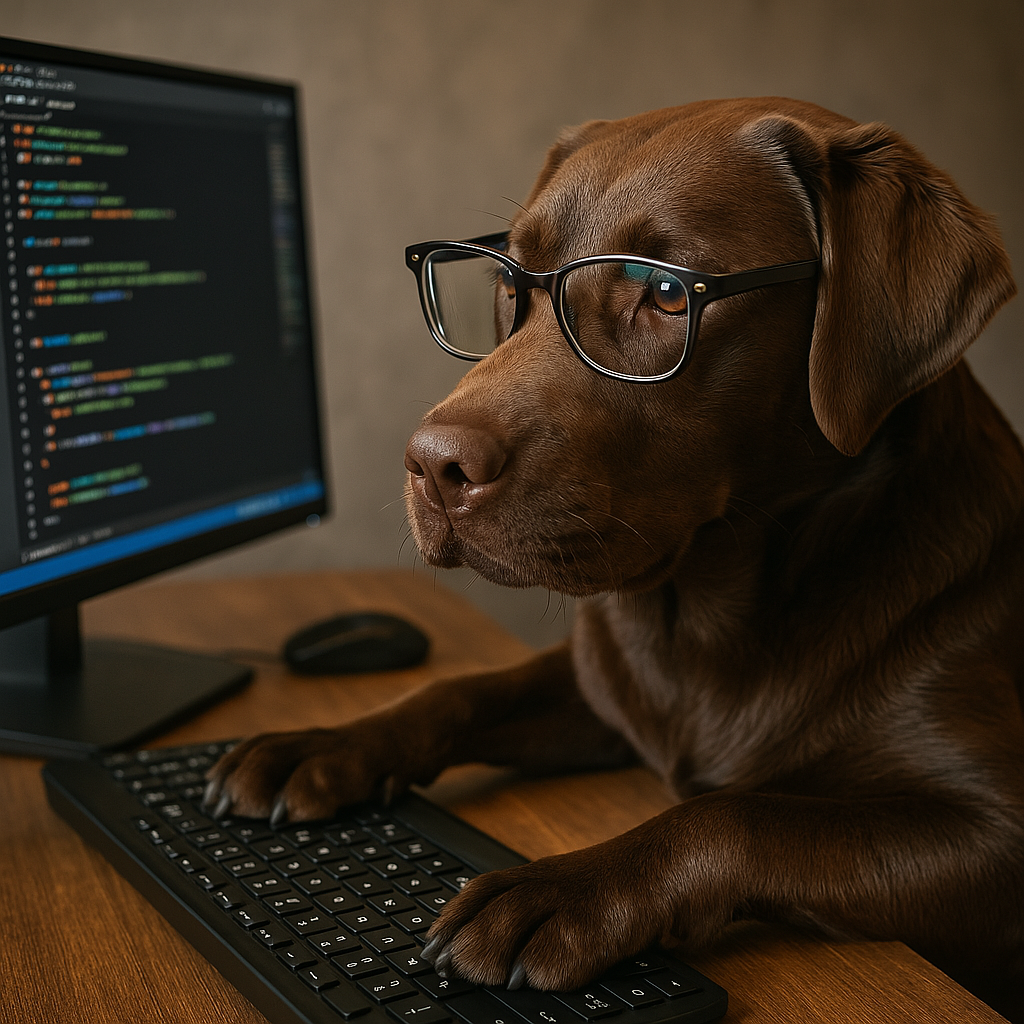
\includegraphics[width=0.5\linewidth]{dissertation//figures/gpt4o.png}
    \caption{An image generated by GPT-4o\cite{4oimagegen} using the prompt ``a chocolate labrador with glasses programming on a computer"}
    \label{fig:gpt4o-dog}
\end{figure}

\subsection{DeepFakes for Malicious Purposes}
\label{sec:mal-deepfakes}

DeepFakes can generate realistic images that are undetectable by humans. When presented with a combination of real and fake videos, individuals were asked to classify them as either real or fake; the overall accuracy was 55.54\%\cite{diel2024human}, only slightly better than guessing. DeepFakes were initially used for entertainment purposes; for example, individuals would use them to add the actor Nicholas Cage to movies he did not originally star in\cite{harris2023deep}. However, DeepFakes soon began to be used for various malicious purposes.

DeepFakes have been used by state actors and opponents to misrepresent candidates in elections across the globe. In the 2016 United States election, Russian-generated fake videos were published on social media to ``undermine public faith in the U.S. democratic process, denigrate Secretary [Hilary] Clinton, and harm her electability and potential presidency"\cite{harris2023deep}. A similar misinformation campaign was attempted by Russia during the 2017 French elections where documents were stolen from Emmanuel Macron's campaign team and edited in an attempt to hinder his chances of being elected\cite{chesney2019deep}. They were unsuccessful in this campaign due to Macron's team's swift action in countering the documents published. 

On an individual scale, DeepFakes are used by scammers to defraud vulnerable people out of their money. A number of celebrities' likenesses have been used to promote products without their consent. Quantum AI is one such DeepFake-based scam\cite{sensity2024state}. DeepFakes videos of celebrities local to the area (such as Rishi Sunak in England or Justin Trudeau in Canada) were DeepFaked and posted to social media, endorsing the tool which guaranteed ``\$3,000 as early as day one". The second phase of the scam involved sockpuppets (non-existent people entirely AI-generated) posing as local media reporting on the fake endorsements, further promoting the scam. Victims are prompted to invest a small amount of money to start with, often receiving genuine returns; soon, however, victims would be locked out of their account with their money stolen.

Another disturbing use for DeepFakes has been around since their inception: pornography. Approximately 96\% of all DeepFakes generated are pornography\cite{ajder2019state}. Long video sequences can be created from a handful of images scraped from an individual's public profiles\cite{chesney2019deep}. The videos generated are humiliating for the victims they depict, making them feel extremely vulnerable. Often, these videos are used to further blackmail victims, threatening to release the videos publicly if the victim does not comply.

\section{DeepFake Detection}

With all the harm DeepFakes can do, it is essential to be able to detect them reliably and accurately. Early DeepFakes were easy to spot, often with warping around facial features and other temporal irregularities\cite{diel2024human}. Unfortunately, DeepFakes have become increasingly realistic and this trend is only set to continue. Taking inspiration from the GAN model (Figure \ref{fig:gan-diagram}), tools were developed to detect DeepFakes using AI. Whilst in the GAN architecture the generator is meant to win, discriminators are being generated to accurately detect DeepFakes. Significant investment and research are being made into DeepFake detection; the US government invested \$22,000,000 into DeepFake detection research with the Media and Semantic Forensics program\cite{harris2023deep}.

\subsection{Traditional Neural Network Detection Methods}
\label{sec:traditional-cnns}

CNNs have been used to detect DeepFakes since the original GAN paper\cite{goodfellow2014generative}. Although CNNs are infinitely customisable with the different choices of layers and connections, often CNN architectures will consist of a backbone and a head\cite{elharrouss2024backbones}. Backbones are large convolutional neural networks that have been pre-trained on a large dataset that can extract features from an input. A custom head is then added to the network to convert the features into the desired output.

In the context of DeepFake detection, the backbone is trained on ImageNet\cite{deng2009imagenet} an image dataset with 3.2 million images. Backbones are initially trained to classify an image in the dataset to an overall class (for example, ``cat"). The backbone is then released with the weights from the training. For DeepFake detection, the head ends with a fully connected layer with a binary softmax (Equation \ref{eq:softmax}) to classify an image as real or fake. Softmax separates an $N$ large input vector $z$ into separate probabilities, representing the probability that an input is in class $y$ such that $\sum^N_{i=1} y_i=1$. 

\begin{equation}
    \label{eq:softmax}
    y_i=\frac{e^{z_i}}{e^{z_1} + e^{z_2}}, i\in1,2
\end{equation}

Using the final weights from a previous problem as the initial weights for a similar new problem is a technique called transfer learning\cite{bozinovski1976influence} and can vastly improve a network's learning time and accuracy. The header's learnable parameters are initialised randomly. To extrapolate image classification to video classification, each frame of the video is independently classified and then the classifications are aggregated. Various aggregation methods exist, but the simplest one is to set a threshold of frames that can be flagged as DeepFaked before the overall video is classified as fake.

Several backbones have been applied to DeepFake detection with varying success\cite{thing2023deepfake}. The first backbones to be applied to DeepFake detection were VGG16/19\cite{simonyan2014very} and ResNet\cite{he2016deep}. VGG is a typical CNN as outlined in Section \ref{sec:cnns}, ResNet introduced the concept of skip connections, allowing for the interaction of high and low level features. 

State-of-the-art backbones have also been applied to DeepFakes, the best performing CNNs are currently based on the EfficientNet\cite{tan2019efficientnet} and Xception\cite{chollet2017xception} backbones. These achieve impressive accuracy on standard benchmarks (Section \ref{sec:datasets}), achieving over 90\% accuracy\cite{bonettini2021video}.

EfficientNet is a model based on the MobileNet\cite{howard2017mobilenets} architecture, which aims to reduce the size of neural networks. EfficientNet is built upon depthwise separable convolutions. A traditional convolutional layer will analyse every channel of an input (such as the red, green, and blue channels in an image) at once, and then combine them in a single step for every pixel in an image. A depthwise separable convolution layer instead analyses each input channel independently and then combines them afterwards. This vastly reduces the computation required as learnable parameters are separated from each other in different stages, as such when combined over larger images the parameters combine linearly rather than exponentially, reducing computation costs. Bottlenecks further speed up EfficientNet by reducing the dimensions of feature vectors. As data flows through a traditional CNN it can reach a large number of dimensions, bottlenecks reduce the dimensions of a neural network which exponentially increases the network's speed. Bottlenecks reduce the dimension by having fewer neurons than the layer before it, forcing data to be aggregated and hence reducing complexity. Whilst MobileNet was intended to reduce the size of CNNs, it can make larger ones more efficient on the same number of parameters. EfficientNet uses MobileNet to allow it to contain more layers and parameters, increasing overall accuracy.

Xception has an architecture similar to ResNet with skip connections. However, rather than direct skips, residual layers pass through a convolution layer to enhance predictions. Furthermore, the same residuals are used in different layers of the network to keep higher-level features in context throughout the network.

CNN detection works by pixel-level analysis of images. Due to the nature of CNNs, it is difficult to tell exactly what features they are focussing on for the final classification. However, thanks to attention layers, it is possible to view the regions of interest (shown in Figure \ref{fig:attention}), implying that the particular areas of attention are the front facial features. Often these will be the areas that DeepFakes will have the hardest time accurately replicating and will often leave artifacts, such as inconsistent shaping\cite{verdoliva2020media}. CNNs are then picking up on these artefacts as markers to classify a DeepFake. This leaves them vulnerable to possible pixel-based attacks which can disrupt the initial feature-extraction\cite{gandhi2020adversarial}. Furthermore, reliance on specific artefacts causes CNNs to only be particularly effective on the DeepFake methodology they were trained and hence suffer reduced accuracy when viewing novel DeepFake methods\cite{thing2023deepfake}.

\begin{figure}[H]
    \centering
    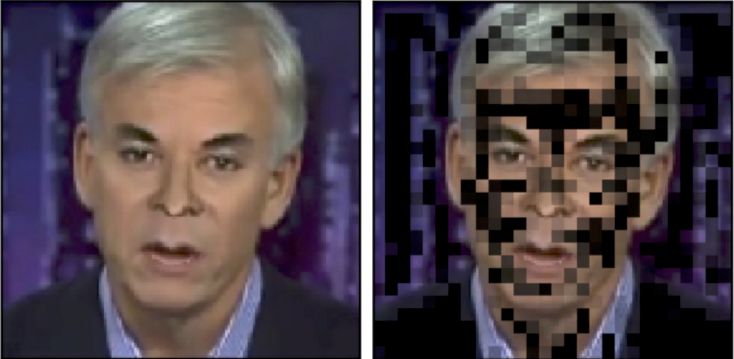
\includegraphics[width=0.5\linewidth]{dissertation//figures/attention-cnns.png}
    \caption{Output from attention layers of convolutional neural networks on DeepFake detection\cite{bonettini2021video}}
    \label{fig:attention}
\end{figure}

\subsection{Blink-Based Detection Methods}
\label{sec:blink-based-detection}

% \begin{itemize}
%     \item Human's blink in a periodic and predictable manner
%     \item DeepFakes struggle with temporal stuff
%     \item Eye Aspect Ratio
%     \item DeepVision
%     \item Ictu Oculi
%     \item see progress report for evaluation and other stuff
% \end{itemize}

DeepFakes have been shown to suffer from temporal inconsistencies\cite{juefei2022countering}. Temporal inconsistencies are where videos suffer from unrealistic deviations between frames. For example, an object in the background may be temporarily obscured by the subject but when they move away from the object, it will have disappeared. 

A more subtle but ever-present temporal consistency is blinking. Humans blink predictably, with the average person blinking for 0.1-0.4 seconds and a 2.8 second blink period\cite{schiffman1990sensation}. These timings can vary according to several factors like age, gender, time of day, and activity\cite{jung2020deepvision}; nevertheless, blinking remains a consistent physiological act that can be predicted, which DeepFakes struggle to reproduce. Blinking patterns can therefore be leveraged for DeepFake classification.

\subsubsection{Eye Aspect Ratio}

To determine when an individual is blinking or not, the most common approach is the Eye Aspect Ratio (EAR)\cite{soukupova2016eye}. The EAR is a ratio of the distance between six eye landmarks (Figure \ref{fig:ear}). Two landmarks are labelled as the caruncle and lateral canthus ($p_1$ and $p_4$, respectively) and the others are equidistant around the eyelid, labelled clockwise. The EAR is the ratio between the height and width of the eye (Equation \ref{eq:ear}) and is relatively constant when the eye is open but verges close to zero when closed. It is partially consistent between people and variations in poses. The modal person has two eyes and so the final EAR is often taken as the average of the two eyes. When plotted as an EAR-time graph (Figure \ref{fig:ear-graph}), a blink is evident as a steep drop in the graph. 

\begin{figure}[H]
    \centering
    \begin{subfigure}{0.45\textwidth}
        \centering
        \begin{tikzpicture}
            \node[anchor=south west, inner sep=0] at (0,0) {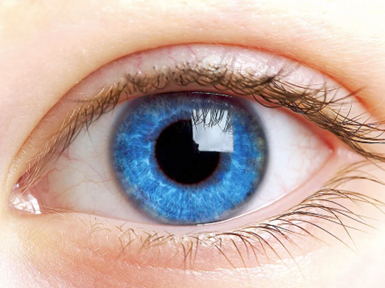
\includegraphics[width=\linewidth]{dissertation/figures/eye.png}};
            \filldraw[black] (0.7,1.7) circle (5pt) node[anchor=west, xshift=5pt] {$p_1$};
            \filldraw[black] (2.2,3.4) circle (5pt) node[anchor=north east, yshift=-5pt] {$p_2$};
            \filldraw[black] (4.6,3.5) circle (5pt) node[anchor=north west, xshift=3pt] {$p_3$};
            \filldraw[black] (6.2,2.6) circle (5pt) node[anchor=east, xshift=-5pt] {$p_4$};
            \filldraw[black] (4.5,1.4) circle (5pt) node[anchor=south west, xshift=4pt] {$p_5$};
            \filldraw[black] (2.8,1.2) circle (5pt) node[anchor=south east, xshift=-3pt] {$p_6$};
        \end{tikzpicture}
        \caption{An image of a human eye with the 6 points necessary for the EAR labelled}
        \label{fig:ear}
    \end{subfigure}
    \hfill
    \begin{subfigure}{0.45\textwidth}
        \centering
        \raisebox{1.8cm}{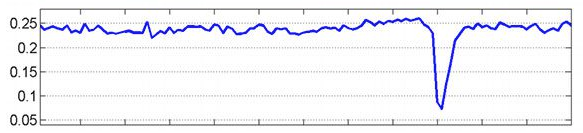
\includegraphics[width=\linewidth]{dissertation/figures/ear-graph.png}}
        \caption{A graph of EAR over time with a blink in the final third \cite{soukupova2016eye}}
        \label{fig:ear-graph}
    \end{subfigure}
    \caption{The points and resulting graph for the Eye Aspect Ratio}
\end{figure}

\begin{equation}
    \label{eq:ear}
    EAR=\frac{||p_2-p_6|| + ||p_3-p_5||}{2||p_1-p_4||}
\end{equation}

\subsubsection{DeepVision}

DeepVision\cite{jung2020deepvision} is a detection model that utilises the EAR and other environmental factors to determine whether a video is DeepFaked or not by comparing its blink patterns to a database of known correct blinking patterns.

DeepVision's input includes not only the video to be classified but also several environmental factors. A user must manually estimate the: gender, age, time, and activity (whether the subject is moving or stationary) of the main subject of the video. 

Two algorithms are used to detect a blink. The first algorithm is a target detector that uses Fast-HyperFace\cite{ranjan2017hyperface} which is a pre-trained CNN that can identify subjects in a video and produce basic landmarks. If the detection confidence is over 70\%, the subject is identified as the target and a basic crop of their face is calculated from the landmarks and forwarded to the next algorithm.

A second algorithm takes the face crops and locates the landmarks ($p_{1-6}$) for the EAR. Whilst the exact method is not defined, it is assumed to be the neural network used in the original EAR paper, Intraface\cite{xiong2013supervised}. From these six points, the EAR is calculated for each eye and then averaged across the two. A blink is defined as when the EAR drops below a certain threshold for multiple consecutive frames. DeepVision sets this threshold as two standard deviations below the mean. Data such as when the blink occurred in time, the period of blink, and frequency are then used as features for the next step.

DeepVision compares these features with known good features from a database. The database was created using data from the Eye Blinking Prediction Dataset\cite{turing2018eye}. The database is queried for individuals in the same environment as the subject and the corresponding features of blinking across the video are returned. The database's features are compared to the video's and if they are ``within an allowable" range the video is declared as real, otherwise fake. DeepVision achieves an overall accuracy of 87.5\%.

\begin{figure}[h]
    \centering
    \begin{subfigure}{0.45\textwidth}
        \centering
        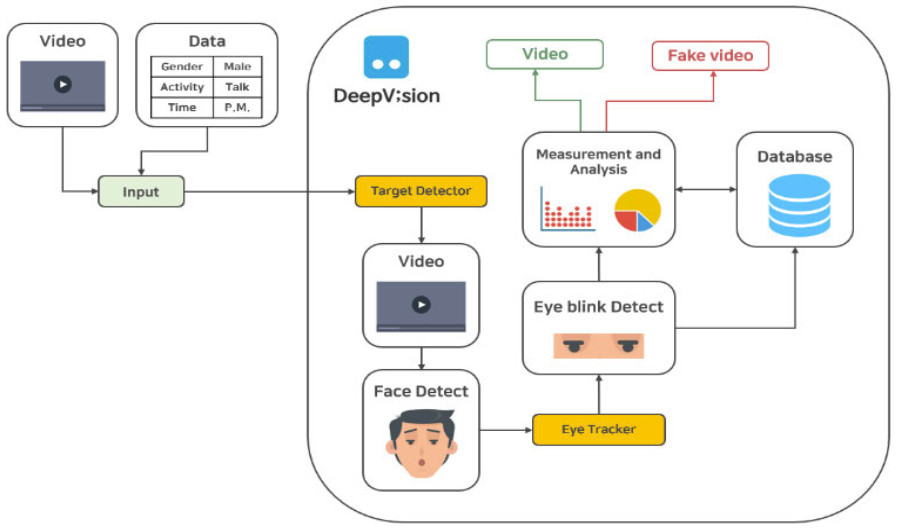
\includegraphics[width=\linewidth]{dissertation//figures/deepvision-flow.png}
        \caption{A flow diagram for DeepVision\cite{jung2020deepvision}}
        \label{fig:deepvision-flow}
    \end{subfigure}
    \hfill
    \begin{subfigure}{0.45\textwidth}
        \centering
        \raisebox{1.2cm}{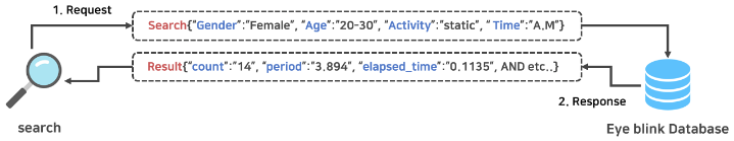
\includegraphics[width=\linewidth]{dissertation//figures/deepvision-database.png}}
        \caption{A sample database query for DeepVision\cite{jung2020deepvision}}
        \label{fig:deepvision-database}
    \end{subfigure}
    \caption{DeepVision's architecture and database queries}
    \label{fig:deepvision}
\end{figure}

DeepVision's primary advantage is that it is easy to compute and implement. Fast-HyperFace is a pre-trained model and therefore is a simple drag-and-drop implementation. Once $p_{1-6}$ are located in a frame, it is a simple calculation to determine the EAR. The subsequent statistical analysis to determine whether blinking is consistent with real videos is also relatively simple and not computationally intensive as it is a database query. Therefore, any methodology utilising DeepVision would be fast to implement and relatively easy to debug. It also benefits from more granularity in eye state data which could enable more complex analysis.

The primary downside to DeepVision is the potential occlusion of the eye(s). The EAR requires the entire eye to be visible in the frame of a video to identify all the points. A partial EAR can be calculated with a single eye, but the accuracy of this is less than if two eyes were visible. The second disadvantage is the database required to determine whether blinking is consistent with normal blinking. The database requires many labelled examples which would be time-consuming to produce. Furthermore, the exact methodology for determining whether a video's data is similar enough to the dataset's is never explained, nor is the ``allowable" range, resulting in DeepVision's accuracy being unlikely to be replicable.

\subsubsection{Ictu Oculi}

Another method for blink-based DeepFake detection is Ictu Oculi\cite{li2018ictu}. It uses a more complex method of blink detection which allows a simple method for blink verification. 

An initial pre-processing step is done to identify the faces of the image using dlib's\cite{king2009dlib} face detector and distort and crop them so that the face is: in the centre of the image; rotated such that the eyes form a horizontal line; and scaled to a similar size across the duration of the video. The face tracked in the video is the one which the network predicts with the highest confidence. This face is further cropped to just the eyes which is then passed to the main model.

To determine the current state of the eye (open or closed), Ictu Oculi uses a custom Recurrent Neural Network (RNN). RNNs are similar to CNNs but contain recurrent connections that can loop backwards through the network, allowing for a form of memory. This makes RNNs very effective for analysing time-based data as each position in time can be predicted using the context of the previous prediction; unlike CNNs, which would analyse each position independently.

The specific form of RNN used by Ictu Oculi is Long Short-Term Memory (LSTM) modules\cite{hochreiter1997long}. LSTM modules dictate how many of the previous states to remember and how much influence the previous states have on the current prediction. Ictu Oculi consists of three main stages. The first stage is feature extraction using a VGG16-based CNN, discriminative features are extracted from the cropped eyes. The features and the previous LSTM's output are fed into an LSTM in the sequence learning stage. This takes temporal features into account to enhance the blink detection; for example, if the previous five frames have all shown the eye in the process of closing, it is likely the current frame will also show the eye closing. The final stage is the state prediction, which uses a dense layer to determine whether the eye is open or closed. The complete diagram is shown in Figure \ref{fig:ictu-oculi}.

\begin{figure}[h]
    \centering
    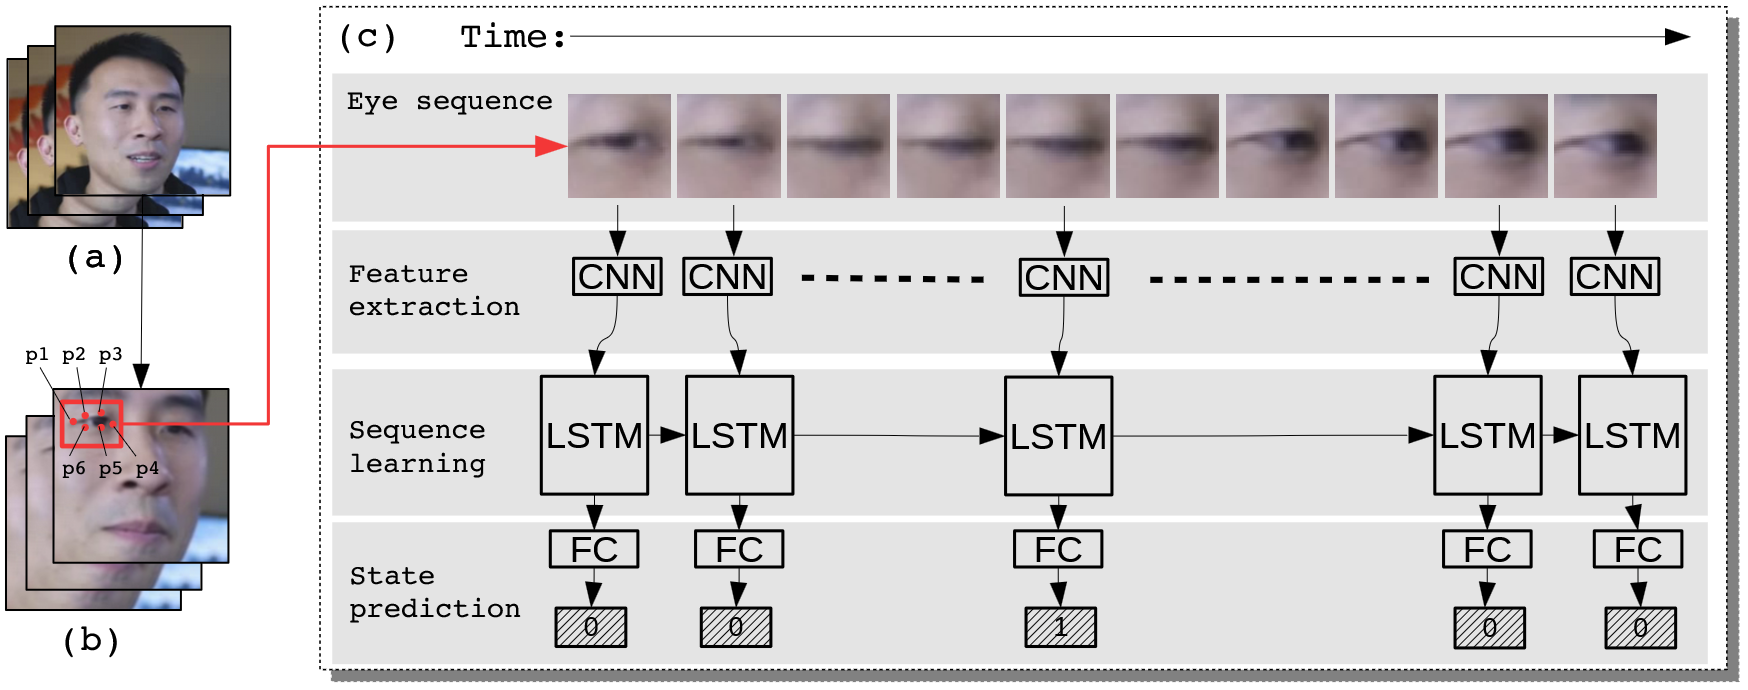
\includegraphics[width=0.75\linewidth]{dissertation//figures/ictu-oculi.png}
    \caption{A network diagram of Ictu Oculi\cite{li2018ictu}}
    \label{fig:ictu-oculi}
\end{figure}

As the accuracy of data is reduced from the amount an eye is open to a binary open or close, the complexity of the validity algorithm needs to be greatly reduced. The algorithm implemented by Ictu Oculi detects the number of blinks in a set period (60 seconds), the average person blinks 34.1 times a minute. A video is deemed fake or real based on how closely the blinking in the video matches this number. This leads to an accuracy of 99\% when tested on a custom dataset of 32 videos.

Ictu Oculi has a much more complex blink detection system, requiring two separate machine learning models trained to identify if a blink is happening or not. This is more complex and requires pre-processing resulting in longer development and training times. On the other hand, it results in a much more resilient blink detection mechanism as the eye's state can be accurately determined even when partially obscured.

The drawback is that the state of the eye is binary open or close, any information relating to the speed of the blink is lost resulting in a very rudimentary system to determine whether a sequence of blinks is a DeepFake or not. Yet, this has little effect on the accuracy of detection.

\section{Adversarial Noise}

% \begin{itemize}
%     \item Additive noise can cause misclassification
%     \item Adversarial Perturbations
%     \item FakeRetouch
%     \item Again see progress report
% \end{itemize}

When operating on images, CNNs heavily rely on the individual pixels in the image. When these pixels are corrupted by noise, it can seriously degrade the performance of CNNs\cite{yim2017enhancing}. For DeepFakes, this noise can cause a misclassification: a fake video could be classed as real, and vice versa. Adversarial noise is deliberate noise added to an image to cause a desirable misclassification. Perturbed images are meant to be imperceptible to humans to avoid manual detection.

Adversarial noise becomes especially dangerous if a CNN is trusted to be accurate. Hypothetically, a CNN is produced that, on unperturbed videos, is 100\% accurate and hence its classifications are trusted absolutely. A malicious actor could add noise to their DeepFake, causing the CNN to declare it real, resulting in the DeepFaked video being trusted as real. Such a scenario is extremely dangerous and so it is important to develop noise-resistant detection models.

\begin{figure}[H]
    \centering
    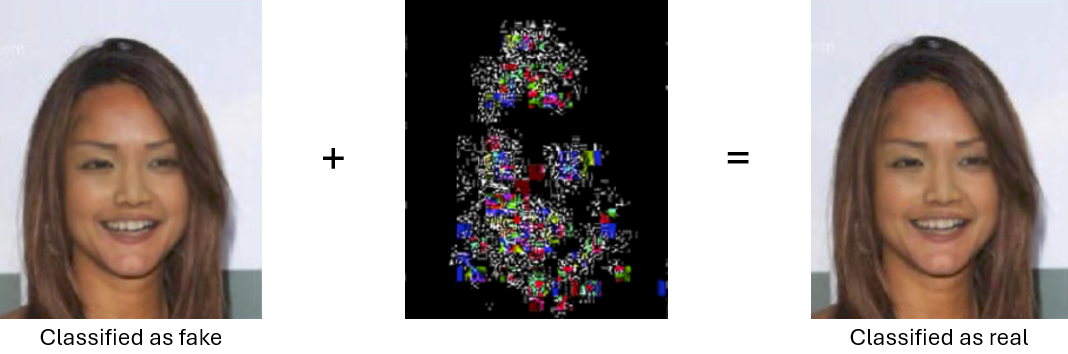
\includegraphics[width=0.75\linewidth]{dissertation//figures/noise.png}
    \caption{The process of adversarial noise being added to an image to cause a misclassification\cite{gandhi2020adversarial}}
    \label{fig:noise}
\end{figure}

There are a large number of methods that have been proven to cause CNNS to misclassify. A smaller subset of these have been proven to be effective in DeepFake classification. It is important to note that adversarial noise is only tested and applied to fake images, as when used in the real world, only the fake videos will be perturbed to make them seem real.

\subsection{Fast Gradient Sign Method}
\label{sec:fgsm}

Fast Gradient Sign Method (FGSM)\cite{goodfellow2014explaining} is the simplest method to add adversarial noise to an image. An image is attacked as follows:

\begin{equation}
    \label{eq:fgsm}
    \mathbf{x}_{adv} = \mathbf{x} + \varepsilon \text{sign}(\nabla_x J(\mathbf{x},\mathbf{y}, \theta))
\end{equation}

$\mathbf{x}_{adv}$ and $\mathbf{x}$ are the perturbed and original frames, respectively. Note that the images are normalised so that $\mathbf{x}_{adv}, \mathbf{x}\in[0,1]^3$. $J(\mathbf{x},\mathbf{y}, \theta)$ is the model's ($\theta$) training loss function on image $\textbf{x}$ and target class $\textbf{y}$. If the model's loss function is not known, it must be guessed; however, most classification models use some form of cross-entropy. Finally, $\epsilon$ is a hyperparameter to control the magnitude of noise. Higher values of $\epsilon$ add more noise to the image, increasing the chance of a misclassification from a CNN, but a similarly higher chance of being detected by humans.

The attack works by estimating the gradient of the loss function for the image $\textbf{x}$. By adding noise in the direction of that loss function, the model becomes less accurate, increasing the risk of misclassification. FGSM is simple and quick to compute as it only requires one call to the CNN being attacked. When tested against DeepFakes, FGSM reduced a ResNet-based detector from 95.4\% accuracy on fake images to 7.5\% accuracy\cite{gandhi2020adversarial}.

\subsection{Carlini-Wagner L2-Norm Attack}

A secondary adversarial noise shown to be effective on DeepFakes is the Carlini-Wagner L2-Norm (CW-L2) attack\cite{carlini2017towards}. It is more complex than FGSM and aims to minimise two objectives: reduce the L2-norm of the noise (Equation \ref{eq:cwl2-2}) while still adding enough noise to cause a misclassification (Equation \ref{eq:cwl2-3}).

\begin{align}
    \mathbf{x}_{adv} &= \frac{1}{2} \left( \tanh(\omega^*) + 1 \right) \label{eq:cwl2-1}\\
    \omega^* &= \arg\min_\omega \left( \|\mathbf{x'} - \mathbf{x}\|_2^2 + c f(\mathbf{x'}) \right) \label{eq:cwl2-2}\\
    f(\mathbf{x'}) &= \max\left( \max_{i \neq y} \left( \mathbf{Z}(\mathbf{x'})_y - \mathbf{Z}(\mathbf{x'})_i \right), -\kappa \right) \label{eq:cwl2-3}
\end{align}

Equation \ref{eq:cwl2-3} aims to cause the model to misclassify an image. $\mathbf{Z}(\textbf{x})$ is the pre-softmax vector output of the neural network, otherwise known as the logits of a model. This allows the CW-L2 attack to analyse the features that a model is using for a prediction rather than the final prediction. $\textbf{x'}$ is a sample perturbed image, $y$ is the index of the target class, and $i$ is the current classification. $\kappa$ acts as a hyperparameter threshold defining the maximum amount the logits can be altered. By minimising $f(\textbf{x'})$, the difference between the logits of the correct class and the target class is maximised, raising the chances of a misclassification.

By minimising the L2-norm of the difference between the original and noisy image in Equation \ref{eq:cwl2-2}, the final noise chosen is the one with the least amount of noise, reducing the chance that humans will detect the noise. $c$ is another hyperparameter that controls the relative strength of each objective. Finally, the noise is normalised to $[0,1]$ in Equation \ref{eq:cwl2-1} to produce the final image.

Often, $c$ is found by a binary search during run time to further minimise the amount of noise on a frame-by-frame basis. To find the argument minimum (Equation \ref{eq:cwl2-2}), SGD\cite{robbins1951stochastic} is used, often with one thousand iteration steps. Both of these result in the CW-L2 attack taking a long time to run in comparison to other methods.

When tested on the same ResNet detector as FGSM (Section \ref{sec:fgsm}), the CW-L2 attack reduced the accuracy on fake videos from 95.4\% to 0\% accuracy. Furthermore, it is more resistant to various noise-reducing filters that may be employed as defence\cite{gandhi2020adversarial}.

\subsection{FakeRetouch}

FakeRetouch\cite{huang2020fakeretouch} is a novel approach to adversarial noise that uses offline-trained CNNs. Instead of targeting a specific model, FakeRetouch aims to reduce a GAN's fingerprints that can show up in the Fourier Transform of an image. As shown in Figure \ref{fig:fakeretouch}, GANs have a much more nosier Fourier transform which some CNNs can leverage as a potential DeepFake identifier. FakeRetouch attempts to minimise the effect a GAN can have on the Fourier transform.

\begin{figure}[H]
    \centering
    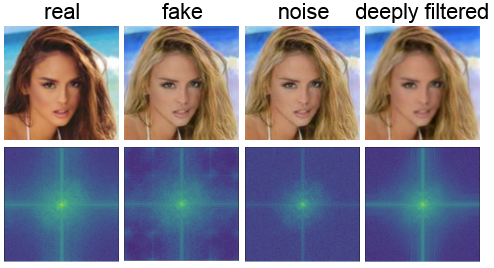
\includegraphics[width=0.5\linewidth]{dissertation//figures/fakeretouch-noise.png}
    \caption{A collection of images and their Fourier Transforms}
    \label{fig:fakeretouch}
\end{figure}

FakeRetouch is defined by the following equation:

\begin{align}
    \mathbf{x}_{adv} &= \mathbf{K} \circledast (\mathbf{x} + \mathbf{A}\odot \mathbf{N}_{\sigma}) \label{eq:fakeretouch-1}\\
    \text{Where } \mathbf{A} &= \arg \max_{\mathbf{A}} \left(J(\mathbf{x}+\mathbf{A},y,\theta)+||\mathbf{A}||_1\right) \label{eq:fakeretouch-2}
\end{align}

$\mathbf{K}$ is a Kernel Prediction Network (KPN)\cite{mildenhall2018burst}. This produces a kernel, similar to the filters in a CNN, that averages out a certain area of pixels to reduce the noise in an image. This can be sufficient for conventional noise reduction but is unfortunately not successful in causing misclassification\cite{huang2020fakeretouch} so further guided noise is required.

FakeRetouch uses Gaussian noise ($\textbf{N}_{\sigma}$) to further blur the image, to reduce the perceptibility of the noise, it is passed through a binary map $\textbf{A}$, which only allows noise in certain regions of the image. It is desirable that $\textbf{A}$ is as sparse as possible to avoid human detection of the noise, hence $\textbf{A}$ is regulated by Equation \ref{eq:fakeretouch-2}. $J$ is the same loss function defined the same as Equation \ref{eq:fgsm} but is set as the categorical cross-entropy loss function. $y$ is the true class label of the image $\textbf{x}$. Equation \ref{eq:fakeretouch-2} regulates the amount of Gaussian noise added to a frame by minimising the L1-norm of the noise.

When tested on DeepFakes, FakeRetouch has limited success. It does not target the neural network directly and so relies on both the neural network analysing the Fourier transform of an image and the DeepFake generator producing excessive fingerprints in the Fourier space. For scenarios where both requirements hold, FakeRetouch can reduce accuracy by 67\%; on the other hand, in scenarios where either one or none of the conditions hold, FakeRetouch either decreases detection by an insignificant amount or can even increase the detection accuracy.

\section{Transferability of DeepFake Detectors}

% \begin{itemize}
%     \item \url{https://arxiv.org/abs/2210.14571}
%     \item CNNs are only effective on the datasets they were trained on, or similar
%     \item real blinking is consistent no matter what the difference is
% \end{itemize}

Another potential flaw with CNN-based DeepFake detectors is their lack of transferability\cite{ricker2022towards} and thus generality. CNNs will often score highly, near 100\% accuracy, on standardised datasets. However, this is often because they have been trained on the same DeepFake methodologies which they are then being tested on. As such, they may have overfitted to recognise the methods on which they have been trained, rather than becoming a generic classifier able to accurately classify unknown DeepFakes.

This problem was demonstrated by Ricker et al.\cite{ricker2022towards}. Three state-of-the-art CNN-based DeepFake detectors were trained on ten datasets each generated using either a GAN or diffusion model. The results are shown in Figure \ref{fig:transferability}. Accuracy is measured using the Probability of detection at a Fixed Alarm Rate (Pd@FAR). As expected, when a model is trained and tested on the same dataset, it achieves close to 100\% accuracy. However, when tested on unknown datasets, a model's accuracy would drop significantly. This effect is more pronounced when models trained on GANs are evaluated on diffusion models, however less so when models trained on diffusion DeepFakes are evaluated against other diffusion DeepFakes. Note in the figure that the GAN, DM, and All columns denote models trained on all GAN-based, Diffusion-based, and all models, respectively.

\begin{figure}[H]
    \centering
    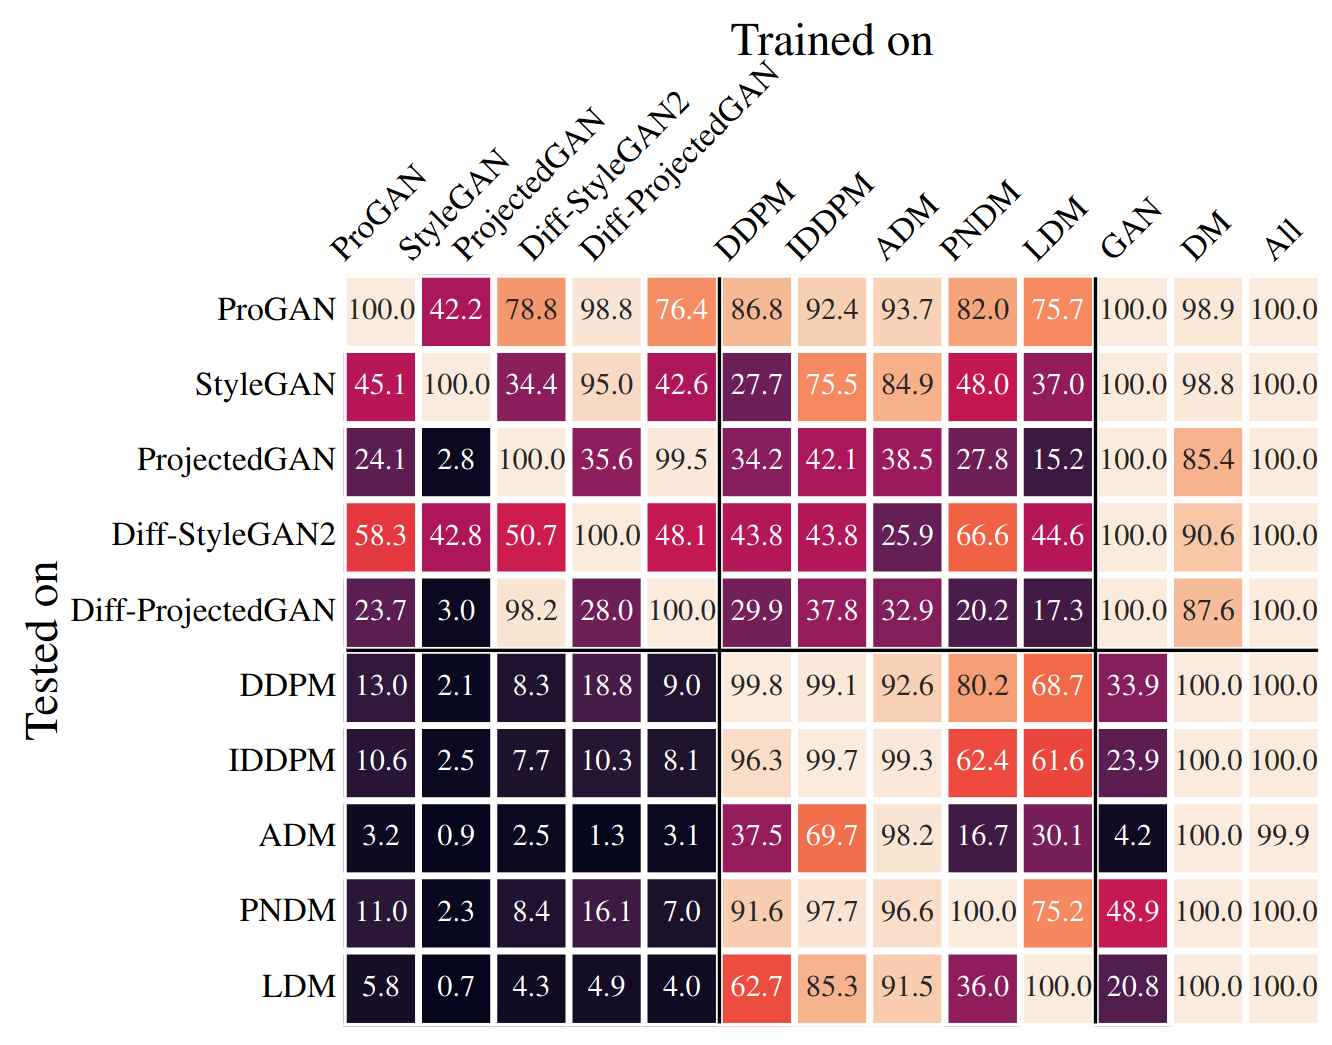
\includegraphics[width=0.75\linewidth]{dissertation//figures/transferability.png}
    \caption{A graph showing the Pd@1\%FAR accuracy of a variety of detection models\cite{ricker2022towards}}
    \label{fig:transferability}
\end{figure}

\section{Datasets}
\label{sec:datasets}

To compare the performance of multiple proposed models, common datasets of DeepFakes have been made. Datasets are large collections of data relevant to a problem that have been collated and labelled by a third party. For DeepFakes, these datasets take the form of videos or images that have been scraped from the internet. These are then passed into at least one DeepFake generator which produces a set of known fake media. This project is only concerned with videos.

FaceForensics++\cite{roessler2018faceforensics}\cite{roessler2019faceforensicspp}\cite{dufour2019deepfakes} is one of the most popular datasets for DeepFake detection on videos. 1,000 images were taken from YouTube and then were DeepFaked with four different methods: Fac2Face\cite{thies2016face2face}, FaceSwap\cite{kowalski2016faceswap}, DeepFakes\cite{deepfakes}, and NeuralTextures\cite{thies2019deferred}. This results in a total of 4,000 videos to train and test classifiers on. 

As part of a 2020 Kaggle competition, Meta released the DeepFake Detection Challenge (DFDC) dataset\cite{dolhansky2020deepfake}. Eight facial modification algorithms were used to create a unique dataset of approximately 124,000 videos. The DFDC is by far the most extensive dataset available. A further testest is also available for use that was not available to participants of the competition although this is not used when benchmarking.

Celebrities are often used in DeepFakes due to their popularity. A number of datasets based on celebrities have been created, these are easier to create as videos involving celebrities are easier to license and larger in number than the typical individual. Celeb-DF\cite{li2020celeb} uses videos of 59 celebrities taken from YouTube. 590 real videos are altered using a custom algorithm to make 5,639 DeepFaked videos. Celebrities were specifically selected to cover a wide range of age, gender, race, and ethnicity. Another dataset that uses videos of celebrities is FakeAVCeleb\cite{khalid2021fakeavceleb}. As the name suggests, it is an audio-visual model, able to fake both the sound and visual components of a video. Similar to CelebDF, videos were deliberately chosen to promote diversity within the dataset. Five hundred videos were altered using four algorithms to create 19,500 videos.

These datasets were chosen for their comprehensive coverage of video-based DeepFake detections. A large number of DeepFake methodologies produce DeepFakes over a wide range of scenarious. Promoting doversity in datasets allows for a more general classifier which will perform better in real-life.